 Let,
\begin{align}
\Vec{A}=\myvec{0 \\ c},
\Vec{B}=\myvec{0 \\ 0},
\Vec{C}=\myvec{a \\ 0}
\end{align}
 Given,
\begin{align}
\ a= 12,
\ b+c = 18
\end{align}
 From  $\triangle ABC$, using  the Baudhayana sutra,
\begin{align}
 b^2 &=c^2+a^2
% \\
% \implies a^2 &=b^2-c^2
% \\
% \implies (12)^2 &=(b+c)(b-c) \quad \brak{\because  a = 12}
% \\
% \implies 144 &=(18)(b-c) 
\\
\implies b-c &=8 \quad \brak{\because b+c = 18}
\end{align}
 Now we have,
\begin{align}
b+c &=18
\\
b-c &=8
\end{align}
which can be expressed as the matrix equation
\begin{equation}
 \myvec{1 & 1\\1 & -1 }\myvec{b\\c} = \myvec{18\\8}
\end{equation}
Applying row reduction, 
\begin{align}
\myvec{
1 & 1   & 18 
\\
1 & -1   & 8 
}
  \xrightarrow{R_2\rightarrow R_2-R_1}
\myvec{
1 & 1   & 18
\\
0 & -2   & -10 
} 
\\
  \xrightarrow{R_1\rightarrow 2R_1+R_2} 
\myvec{
2 & 0   & 26 
\\
0 & -2   & -10 
}
 \xrightarrow[R_2 \rightarrow -\frac{R_2}{2}]{R_1\rightarrow \frac{R_1}{2}} 
\myvec{
1 & 0   & 13 
\\
0 & 1   & 5 
}
\end{align}
Therefore,
\begin{align}
\myvec{b\\c} = \myvec{13\\5}
\end{align}
Thus, 
\begin{align}
\vec{A}=\myvec{0\\c}=\myvec{0\\5}, \vec{B}=\myvec{0\\0}, \vec{c}=\myvec{a\\0}=\myvec{12\\0} 
\end{align}
and  $\triangle ABC$ is plotted in Fig. \ref{constr/6/fig:right_angle_triangle}	
%
\begin{figure}[!ht]
\centering
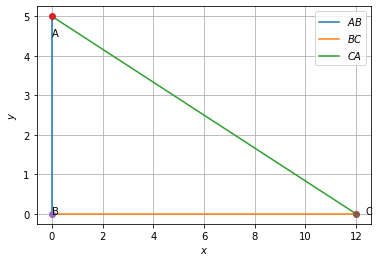
\includegraphics[width=\columnwidth]{solutions/6/figure1.png}
\caption{Right Angle $\triangle ABC$}
\label{constr/6/fig:right_angle_triangle}	
\end{figure}